%% This file is a portion of the source for Revised Edition 1.1 of
%% Operating Systems and Middleware: Supporting Controlled
%% Interaction, Copyright 2011 by Max Hailperin.  This work is
%% licensed under the Creative Commons Attribution-ShareAlike 3.0
%% Unported License. To view a copy of this license, visit
%% http://creativecommons.org/licenses/by-sa/3.0/ or send a letter to
%% Creative Commons, 171 Second Street, Suite 300, San Francisco,
%% California, 94105, USA.
\chapter{Messaging, RPC, and Web Services}
\label{distmid-chapter}

\section{Introduction}

Application programmers who create distributed systems of
communicating processes fundamentally rely upon the support for
networking provided by operating systems;
this support was described in Chapter~\ref{networking-chapter}.
Sometimes this reliance is direct;
for example, the application programs may use sockets to open
connections between TCP ports and then send byte streams that encode
application messages.  Increasingly, however, this reliance is
indirect because a middleware layer comes
between the application program and the socket API.  The application
programmer works in terms of the middleware-supported abstractions,
such as message queues and remotely accessible objects.  The
middleware provides those abstractions by making use of the more
fundamental operating system--supported facilities.

In this chapter, I will present two distinct styles of communication
middleware.  Messaging systems, discussed in
Section~\ref{messaging-section}, support the one-way transmission of
messages.  Application programmers can choose to use those messages in
request-response pairs, but the middleware remains oblivious to this
pairing and treats each message individually.  Sending a request and
receiving a response happen in separate transactions, potentially at
quite different times.  For more tightly coupled interactions, Remote
Procedure Call (RPC) systems provide an alternative style of
communication, as presented in Section~\ref{RPC-section}.
Each time a process invokes an RPC operation, it sends a request and
then immediately waits for a response as part of the same
transaction.  The RPC system makes the request-response pair appear to
the application program as a normal procedure call and return.

After presenting each of these styles of communication, I turn in
Section~\ref{web-services-section} to their connection with web
services.  Web services use standardized communication mechanisms to
make programmed functionality available over the Internet.  Most web
services fit the RPC model, though they can also use one-way messaging
or (in theory) more general message exchange patterns.

Finally, the chapter concludes, as usual, with a look at security
issues in Section~\ref{distmid-security-section} and then exercises,
projects, and notes.

\section{Messaging Systems}\label{messaging-section}

Applications based on one-way transmission of messages use a form of
middleware known as \vocabs{messaging system} or
\foldvocab{message-oriented}{middleware} (\vocab{MOM}).  One popular
example of a messaging system is IBM's WebSphere MQ, formerly known as
MQSeries.  One popular vendor-neutral API for messaging is the Java
Message Service (JMS), which is part of J2EE.

Messaging systems support two different forms of messaging:
\vocab{message queuing} and \vocab{publish/subscribe messaging}.  I
already introduced message queuing in
Section~\ref{transactions-message-queuing-systems-section}.  Here I
will build on that introduction to message queuing and also
provide an introduction to publish/subscribe messaging.

Figure~\ref{scan-10-1} illustrates the difference between the two
forms of messaging.
\begin{figure}
\centerline{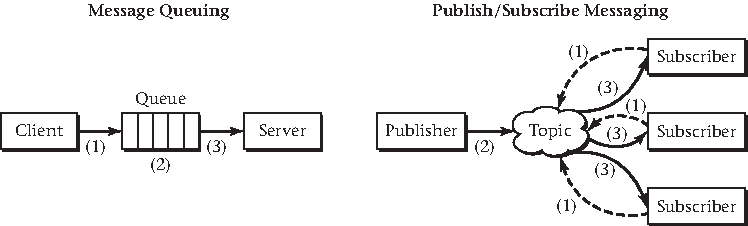
\includegraphics{hail_f1001}}
%\centerline{\def\epsfsize#1#2{0.6#1}\epsfbox{scan-10-1.eps}}
\caption{Message queuing involves three steps: (1) the client sends a
message to a queue, (2) the queue retains the message as long as
necessary, (3) the server retrieves the message.  Publish/subscribe
messaging involves a different sequence of three steps: (1) each subscriber
subscribes with one of the messaging system's ``topic'' objects, (2) the
publisher sends a message to the topic, (3) the message is
distributed to all current subscribers.}
\label{scan-10-1}
\end{figure}
Message queuing strongly decouples the timing of the client and the
server, because the queue will retain the messages until they are
retrieved.  (Optionally, the client can specify an expiration time for
unretrieved messages.)  The server need not be running at the time a
message is sent. On the other hand, the client is only weakly
decoupled from the server's identity. Although the client doesn't send
the message to a specific server, it does send it to a specific queue,
which still creates a \vocab{point-to-point} architectural structure, because each
queue normally functions as the in-box for a particular server.  A
point-to-point structure means that if the
message is of interest to multiple servers, the client needs to
send it to multiple queues.  The publish/subscribe architecture, in
contrast, strongly decouples publishers from any knowledge of the
subscribers' identities.  Each message is sent to a general topic and
from there is distributed to any number of subscribers that have
indicated their interest in the topic.  However, publish/subscribe
messaging usually does not strongly decouple timing.  Messages are usually only
sent to current subscribers, not retained for future subscribers.

The portion of a messaging system managing topic objects for
publish/subscribe messaging is known as a \vocab{broker}.  The broker
is responsible for maintaining a list of current subscribers for each
topic and for distributing each incoming publication to the current
subscribers of the publication's topic.

Section~\ref{transactions-message-queuing-systems-section} explained
the relationship between message queuing and transactions.  A
transaction can retrieve messages from queues, do some processing, such
as updating a database, and send messages to queues.  When the
transaction commits, the input messages are gone from their queues,
the database is updated, and the output messages are in their queues.
If the transaction aborts, then the input messages remain in their
queues, the database remains unchanged, and the output messages have
not entered their queues.

This transactional nature of message queuing has an important
consequence for systems in which request messages are paired with
response messages and will help me explain the difference between
messaging and RPC systems.  Consider a client and server coupled
through request and response queues, as shown in
Figure~\ref{scan-10-2}.
\begin{figure}
\centerline{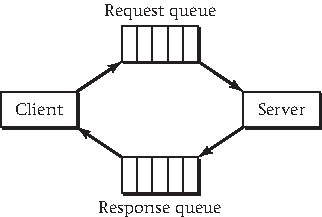
\includegraphics{hail_f1002}}
%\centerline{\def\epsfsize#1#2{0.6#1}\epsfbox{scan-10-2.eps}}
\caption{A client and server can engage in a request-response protocol
  using two message queues.  Typically, the client tags each request
  message with a unique identifying string, known as a
  \vocab{correlation ID}.  The server copies this ID into the
  resulting response message so that the client knows to which request
  the response corresponds.}
\label{scan-10-2}
\end{figure}
The client can generate a request message in one transaction and then
in a second transaction wait for a response message.  However, it
cannot do both in a single transaction, or it will wait forever,
having deadlocked itself.  Until the transaction commits, the request
message doesn't enter the request queue. As a result, the server has
nothing to respond to and won't generate a response message.
Therefore, the client will continue waiting for the response message
and so the transaction won't commit, completing the deadlock.  If
your goal is to have the client make use of the server as one
indivisible step within a transaction, then you need to use RPC rather
than messaging.

Publish/subscribe messaging can participate in transactions as well,
but the results are less interesting.  Publishing is just like sending
to a queue, in that the message isn't actually sent until the
transaction commits.  However, receipt of messages by subscribers is
handled differently.  If a subscriber receives a message within a
transaction and then aborts the transaction, it cannot count on the
message being redelivered when the transaction is retried.

In either messaging model, a consumer may want to receive only
selected messages that are of interest to it.  For example, it may
want to receive stock ticker messages with updated prices, but only
for IBM stock and only if the price is less than 75 or more than 150.
The program could receive all stock ticker messages (by reading from a
queue to which they are sent or by subscribing to a topic to which
they are published) and ignore those that are uninteresting.
However, for the sake of efficiency, messaging systems generally
provide mechanisms to do the filtering prior to message delivery.

In the publish/subscribe model, the selection of just IBM stock might
be accomplished simply by having a sufficiently specific topic.
Messaging systems generally allow topics to be hierarchically
structured, much like files in directory trees or Internet domains
within the DNS.  Thus, a topic for IBM stock prices might be
\verb|finance/stockTicker/IBM|.  A subscriber interested only in this
one stock could subscribe to that specific topic, whereas a subscriber
interested in all stock prices could subscribe to
\verb|finance/stockTicker/+|, where the wildcard \verb|+| indicates
any one subtopic.  Another wildcard, \verb|#|, is fancier than needed
in this case but can be useful in other circumstances.  A
subscription to \verb|finance/stockTicker/#| would receive not only
messages about each individual stock, such as IBM, but also general
messages, directed to \verb|finance/stockTicker| itself, and more
specialized messages, directed to descendant subtopics any number of
levels below \verb|finance/stockTicker/IBM| and its siblings.

This hierarchy of topics is limited, however.  It fits the
publish/subscribe model but not the message queuing  model, and
it addresses only
qualitative selection criteria that naturally lead to distinct
topics.  In the example I gave earlier, it is unlikely that a system
architect would create three subtopics of \verb|IBM| for
\verb|under75|, \verb|between75and150|, and \verb|over150|.  Among
other reasons, there may be other subscribers interested in other price
ranges.

Therefore, messaging systems allow message consumers to specify more general selection
criteria.  In the JMS API,  for example, if \verb|s| is a messaging
\verb|Session| and \verb|d| is a messaging \verb|Destination|, that
is, either a \verb|Queue| or a \verb|Topic|, then executing
\begin{verbatim}
s.createConsumer(d, "Symbol = 'IBM' AND " +
                    "(Price < 75 OR Price > 150)")
\end{verbatim}
will produce a \verb|Consumer| object with the specified selector.
Any \verb|receive| operation performed on that \verb|Consumer| (or any
\verb|MessageListener| registered with that \verb|Consumer|) will see
only those messages satisfying the selection criterion.

\section{Remote Procedure Call}\label{RPC-section}

The goal of \vocab{Remote Procedure Call} (\vocab{RPC}) middleware is
to make request-response communication as straightforward for
application programmers to program as ordinary procedure calls.  The
client application code calls a procedure in the ordinary way, that is, passing
in some arguments and obtaining a return value for its further use.
The procedure it calls just happens to reside in a separate server.
Behind the scenes, the middleware encodes the procedure arguments into
a request message and extracts the return value from the response
message.  Similarly, the server application code can take the form of
an ordinary procedure.  By the time it is invoked, the procedure
arguments have already been extracted from the request message,
freeing it from that responsibility.
Section~\ref{RPC-generalities-section} explains further the
principles upon which RPC operates.  Section~\ref{RMI-example-section}
provides a concrete example of using RPC in the particular form of
Java RMI (Remote Method Invocation).  The subsequent section,
\ref{web-services-section}, is devoted to web services but also
provides additional information on how RPC plays out in that context.

\subsection{Principles of Operation for RPC}\label{RPC-generalities-section}

To understand how RPC middleware functions, it is helpful to
think about the fact that different procedures can present the same
interface.  For example, consider procedures for squaring a number.
You could have several different procedures that take a numeric
argument, compute the square, and return it.  One might work by
multiplying the number by itself.  Another might use a fancy
calculation involving logarithms.  And a third might open up a network
instant-messaging connection to a bored teenager, ask the teenager
what the square of the number is, then return the value it receives,
correctly extracted from the textual instant-messaging response.  This
third procedure is known as a \vocab{proxy} for the teenager.  The
proxy's method of squaring the number involves neither multiplication
nor logarithms, but rather delegation of responsibility.  However, the
proxy still is presenting the same interface as either of the other
two procedures.

Figure~\ref{scan-10-3} shows how RPC middleware uses a proxy to
put the client in the position of making a normal procedure call.  The
client application code actually does make a normal procedure call;
that much is no illusion.  However, it only gives the illusion of
calling the server procedure that does the real computation.  Instead,
the called procedure is a proxy standing in for the server procedure;
the proxy is often known as a \vocab{stub}.  The stub proxy discharges
its responsibility not by doing any actual computation itself, but by
using request and response messages to communicate with the server.
\begin{figure}
\centerline{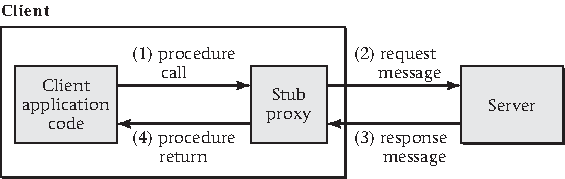
\includegraphics{hail_f1003}}
%\centerline{\def\epsfsize#1#2{0.6#1}\epsfbox{scan-10-3.eps}}
\caption{In Remote Procedure Call, application code makes a normal
  procedure call to a stub proxy, which doesn't carry out the
  requested computation itself, but rather sends a request message to
  the server and then turns the response message into the procedure
  return value.}
\label{scan-10-3}
\end{figure}

The stub proxy suffices to hide communication issues from the
application programmer writing the client code.  In some cases, that
is all that is needed, and the server is written by a networking
expert who can directly write code to handle request and response
messages.  More typically, however, the server code is written by
another application programmer who appreciates middleware support.
As shown in Figure~\ref{scan-10-4},
\begin{figure}
\centerline{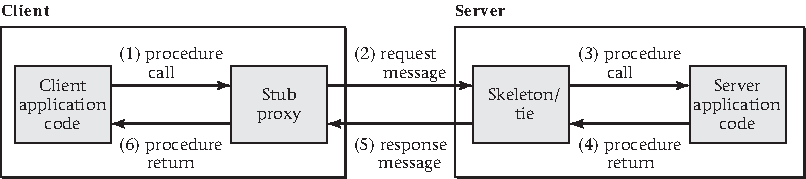
\includegraphics{hail_f1004}}
%\centerline{\def\epsfsize#1#2{0.6#1}\epsfbox{scan-10-4.eps}}
\caption{In order for the server application code to be free from
  communication details, it can be a normal procedure invoked by a
  portion of the RPC runtime sometimes called a skeleton or a tie.}
\label{scan-10-4}
\end{figure}
the server application code can be a
normal procedure, called the same way it would be if it were running
on the same machine with the client.  Once again, the illusion is only
partial.  The server application code really is being called with an
ordinary procedure call.  The only illusion concerns what code is
doing the calling.  From an application standpoint, the caller seems
to be the client.  However, the caller really is a dedicated portion of the
RPC runtime system, known as a \vocab{skeleton} or a \vocab{tie},
the purpose of which is to call the procedure in response to the
request message.  See Figure~\ref{scan-10-5} for the application
programmer's view of the result; the middleware communication
disappears from view and the client application code seems to be
directly calling the server application procedure, as though they were
part of a single system.
\begin{figure}
\centerline{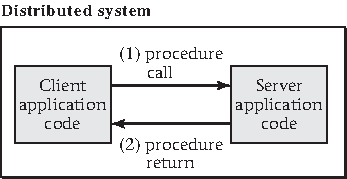
\includegraphics{hail_f1005}}
%\centerline{\def\epsfsize#1#2{0.6#1}\epsfbox{scan-10-5.eps}}
\caption{The application programmer's view of an RPC system has the
  client code apparently making a direct call to the server procedure;
  the RPC proxy mechanism is invisible.}
\label{scan-10-5}
\end{figure}

Early versions of the RPC communication model were based on ordinary
procedure calls, whereas more recent versions are based on the
object-oriented concept of method invocation.  The basic principles
are the same, however, and the name RPC is commonly understood to
include method invocation as well as procedure calling.

A key example of a non-object-oriented RPC standard is Open Network
Computing (ONC) RPC, which was developed at Sun Microsystems and
became an Internet standard.  ONC RPC serves as the foundation for
NFS, the Network File System discussed in Section~\ref{dfs-section}.
Each NFS operation, such as reading from a file, is carried out by
calling an RPC stub procedure, which takes responsibility for
packaging the procedure arguments into a request message and for
extracting the return value from the response message.

In object-oriented versions of RPC, the stub proxy is an object
presenting the same interface as the server object.  That is, the same
repertoire of methods can be invoked on it.  The stub uses a
uniform strategy for handling all methods: it translates method
invocations into appropriate request messages.

Two significant object-oriented RPC standards are \vocab{CORBA} and
\vocab{RMI}.  CORBA (\vocab{Common Object Request Broker Architecture}) is a
complicated language-neutral standard that allows code written in one
language to call code written in another language and located
elsewhere in a distributed system.  RMI (\vocab{Remote Method
  Invocation}) is a considerably simpler
mechanism included as part of the Java
standard API; part of its simplicity comes from needing to
support only a single programming language.  Because RMI can optionally use
CORBA's communication protocol, the Internet Inter-ORB Protocol
(IIOP), the two systems can interoperate.

One important feature of object-oriented RPC systems such as RMI is
that the values communicated as method arguments and return values can
include references to other objects.  That is, a remotely invoked
method can operate not only on basic values, such as integers or
strings, but also on user-defined types of objects.  One
remotely accessible object can be passed a reference that refers to another
remotely accessible object.  In fact, this is the way most objects find
out about other objects to communicate with after getting past an
initial startup phase.

To initially get communication started, client objects typically look
up server objects using a \vocab{registry}, which is a specialized
server that maintains a correspondence between textual names and
references to the remotely accessible objects.  (These correspondences
are known as \vocab{bindings}.)  The registry itself can be located,
because it listens for connections on a prearranged port.  When an
application server object is created that a client might want to
locate, the server object is bound to a name in the registry.  The
client then presents the same textual name to the registry in a lookup
operation and thereby receives a reference to the initial server
object it should contact.

After this initial contact is made, the objects can use the arguments
and return values of remote method invocations to start passing each
other references to additional objects that are not listed in the
registry.  Pretty soon any number of client and server objects can
have references to one another and be invoking methods on each other.

Section~\ref{RMI-example-section} is occupied by an RMI programming
example designed to reinforce the aforementioned point, that remote
objects are located not only using the registry, but also by being
passed as references. This example illustrates the way in which an
application programmer uses RMI and thereby complements the preceding
general discussion of how RPC stubs and skeletons work.  I do not
provide any more detailed information on the inner workings of RMI.
However, in Section~\ref{web-services-section}, I show the how RPC
messages are formatted in the web services environment.

\subsection{An Example Using Java RMI}\label{RMI-example-section}

Using RMI, it is possible to develop an implementation of the
publish/subscribe messaging model, in which publishers send messages
to topic objects, which forward the messages along to subscribers.
The code in this section shows such an implementation in the simplest
possible form.  In particular, this code has the following limitations;
to address each limitation, there is at least one corresponding Programming Project:
\begin{itemize}
\item
The message delivery is fully synchronous.  That is, the publisher asks
the topic object to deliver a message; control does not return to the
publisher until the message has been delivered to all the subscribers.
Programming Projects \ref{BoundedBuffer-TopicServer-project} and
\ref{Spawning-TopicServer-project} address this.
\item
The example programs support only a single topic.  Programming
Projects \ref{registered-topics-project} and
\ref{multi-topic-server-project} address this.
\item
In the example code, there is no way for a subscriber to explicitly
unsubscribe from a topic.  However, the code does support subscribers
that terminate, lose communication, or otherwise fail.  Programming
Project~\ref{unsubscribe-project} provides explicit unsubscription.
\item
The example code includes simple command-line interfaces for sending
textual strings as messages and for displaying received messages on
the terminal.  These suffice to demonstrate the communication but do
not have the appeal of a chat-room application or multi-player game.
Programming Project~\ref{chat-room-game-project} provides the opportunity
to address this shortcoming.
\end{itemize}

When using RMI, each object that is remotely accessible must implement
a Java interface that extends {\tt java.rmi.Remote}.  Each method in
that interface must be declared as potentially throwing {\tt
java.rmi.RemoteException}.  This potential for an exception is
necessary because even if the underlying operation cannot possibly
fail, the remote invocation of that operation can fail in myriad ways,
such as through a network disconnection or a crash of the machine on which
the remote object is located.  Figure~\ref{MessageRecipient-source}
shows the source code for a simple remote interface implemented by
subscribers and also by topic objects.  The reason why these two
categories of participants in the publish/subscribe model
implement this same interface is that they have something in common:
they both receive messages.
\begin{figure}
\begin{verbatim}
import java.rmi.Remote;
import java.rmi.RemoteException;

public interface MessageRecipient extends Remote {
  void receive(String message) throws RemoteException;
}
\end{verbatim}
\caption{The {\tt MessageRecipient} interface describes the common
  feature shared by subscribers and the central topic objects that
  redistribute published messages to subscribers: any of these objects
  can receive a message.}\label{MessageRecipient-source}
\end{figure}

Subscribers directly implement the {\tt MessageRecipient}
interface, as you will see later.  However, topic objects need to
implement an extension of the interface, because they can do
more than receive messages; they can also add subscribers.
Figure~\ref{Topic-source} shows the {\tt Topic} interface, which
extends {\tt MessageRecipient} through the addition of a {\tt
  addSubscriber} method.  Notice that the argument passed to {\tt
  addSubscriber} is itself a {\tt MessageRecipient}.  This allows a
reference to one remotely accessible object (the subscriber) to be
passed to another (the topic) for its later use.
\begin{figure}
\begin{verbatim}
import java.rmi.RemoteException;

public interface Topic extends MessageRecipient {
  void addSubscriber(MessageRecipient subscriber)
    throws RemoteException;
}
\end{verbatim}
\caption{The {\tt Topic} interface provides an operation for
  subscribers to use to register their interest in receiving messages.
  By extending the {\tt MessageRecipient} interface, the {\tt Topic}
  interface is also prepared to receive messages from publishers.}\label{Topic-source}
\end{figure}

Having seen these two interfaces for remotely accessible objects, you
are now ready to see an example of code that makes use of such an
object.  Figure~\ref{Publisher-source} contains a simple program for
sending a textual message (given as the first command-line argument)
to a remote object implementing the {\tt Topic} interface.  The
specific remote object is looked up with the aid of a registry, that is, a service
within RMI that records name/object bindings.  The registry is
located on a server computer whose hostname is specified as the second
command-line argument or on the local computer if no hostname is given.
\begin{figure}
\begin{verbatim}
import java.rmi.registry.LocateRegistry;
import java.rmi.registry.Registry;

public class Publisher {

  public static void main(String[] args) {
    if(args.length < 1 || args.length > 2){
      System.err.println("Usage: java Publisher message [host]");
      System.exit(1);
    }
    String message = args[0];
    String hostname = args.length > 1 ? args[1] : null;
    try {
      Registry registry = LocateRegistry.getRegistry(hostname);
      Topic topic = (Topic) registry.lookup("topic.1");
      topic.receive(message);
    } catch (Exception e) {
      System.err.println("caught an exception: " + e);
      e.printStackTrace();
    }
  }
}
\end{verbatim}
\caption{This program uses the registry to locate the remote object
  that is named {\tt topic.1} and that
  implements the {\tt Topic} interface.  The program then asks that
  object to receive a message.}\label{Publisher-source}
\end{figure}

Let's turn next to an example of how a remotely accessible object can
be created and listed in the registry.  The {\tt Topic Server} class,
as shown in Figures \ref{TopicServer-source1} and \ref{TopicServer-source2}, implements the {\tt Topic}
interface.  Each {\tt TopicServer} keeps track of its current
subscribers; additions happen in the {\tt addSubscriber} method, and
deletions happen when a message cannot be successfully delivered.
Because the RMI infrastructure is allowed to invoke each operation in its own
thread, the remote operations
are marked as {\tt synchronized} so as to provide mutual exclusion.
This prevents any races in the manipulations of the list of subscribers.
When the {\tt TopicServer} program is run from the command line, the
{\tt main} method creates an instance of the class, exports it for
remote access, and places it in the local registry, using the same
{\tt topic.1} name as the {\tt Publisher} class looks up.
\begin{figure}
\begin{verbatim}
import java.rmi.registry.Registry;
import java.rmi.registry.LocateRegistry;
import java.rmi.RemoteException;
import java.rmi.server.UnicastRemoteObject;
import java.util.List;
import java.util.ArrayList;

public class TopicServer implements Topic {

  private List<MessageRecipient> subscribers;

  public TopicServer(){
    subscribers = new ArrayList<MessageRecipient>();
  }

  public synchronized void receive(String message)
    throws RemoteException
  {
    List<MessageRecipient> successes =
      new ArrayList<MessageRecipient>();
    for(MessageRecipient subscriber : subscribers) {
      try {
        subscriber.receive(message);
        successes.add(subscriber);
      } catch(Exception e) {
        // silently drop any subscriber that fails
      }
    }
    subscribers = successes;
  }
\end{verbatim}
\caption{The {\tt TopicServer} class continues in the Figure~\ref{TopicServer-source2}.
  The {\tt receive} method shown here is remotely invoked
  by publishers and itself remotely invokes the {\tt receive} method
  of subscribers.}\label{TopicServer-source1}
\end{figure}
\begin{figure}
\begin{verbatim}
  public synchronized void addSubscriber(MessageRecipient subscriber)
    throws RemoteException
  {
    subscribers.add(subscriber);
  }

  public static void main(String args[]) {
    try {
      TopicServer obj = new TopicServer();
      Topic stub =
        (Topic) UnicastRemoteObject.exportObject(obj, 0);
      Registry registry = LocateRegistry.getRegistry();
      registry.rebind("topic.1", stub);
      System.err.println("Server ready");
    } catch (Exception e) {
      System.err.println("Server exception: " + e.toString());
      e.printStackTrace();
    }
  }
}
\end{verbatim}
\caption{This continuation of the {\tt TopicServer} class, begun in Figure~\ref{TopicServer-source1},
  shows how remote objects are
  created, exported (that is, made remotely accessible), and bound to a
  name in the registry.}\label{TopicServer-source2}
\end{figure}

The final component of the example publish/subscribe system is the
{\tt Subscriber} class, as shown in Figure~\ref{Subscriber-source}.
This class provides a simple test program which displays all the
messages it receives.  Like the {\tt Publisher} class, it uses the
registry on a specified host or on the local host if none is specified.
Also like the {\tt Publisher} class, it looks up the name {\tt
  topic.1} in that registry, thereby obtaining a reference to some
remote object implementing the {\tt Topic} interface.  
The reference will actually be to
a proxy that implements the interface.  However, the
proxy will be communicating with an instance of the {\tt TopicServer}
class.  Unlike the {\tt Publisher}, the {\tt Subscriber} is itself a
remotely accessible object.  It is created and exported just like the
{\tt TopicServer} is.  However, it is not bound in the registry; the
{\tt TopicServer} does not locate its subscribers by name.
\begin{figure}
\begin{verbatim}
import java.rmi.registry.LocateRegistry;
import java.rmi.registry.Registry;
import java.rmi.RemoteException;
import java.rmi.server.UnicastRemoteObject;

public class Subscriber implements MessageRecipient {

  public synchronized void receive(String message)
    throws RemoteException
  {
    System.out.println(message);
  }

  public static void main(String[] args) {
    if(args.length > 1){
      System.err.println("Usage: java Subscriber [hostname]");
      System.exit(1);
    }
    String hostname = args.length > 0 ? args[0] : null;
    try {
      Registry registry = LocateRegistry.getRegistry(hostname);
      Topic topic = (Topic) registry.lookup("topic.1");
      Subscriber obj = new Subscriber();
      MessageRecipient stub = (MessageRecipient)
        UnicastRemoteObject.exportObject(obj, 0);
      topic.addSubscriber(stub);
    } catch (Exception e) {
      System.err.println("caught an exception: " + e);
      e.printStackTrace();
    }
  }
}
\end{verbatim}
\caption{Instances of the {\tt Subscriber} class are created and
  exported the same way as {\tt TopicServer}s are, so that they can be
  remotely accessed.  However, they are not bound in the registry.
  Instead, the stub referring to the {\tt Subscriber} is passed to the {\tt addSubscriber}
  method so the {\tt TopicServer} can store the reference away for later.}\label{Subscriber-source}
\end{figure}

Before you can successfully run the {\tt
TopicServer} and test it using the {\tt Publisher} and {\tt
Subscriber} programs, you will probably need to run the {\tt rmiregistry} program that comes
as part of the Java system.  The details of how you run this program are
system-specific, as is the mechanism for ensuring that all components
of the overall RMI system have access to your classes.  Therefore, you
are likely to need to consult the documentation for your specific Java
system in order to successfully test the sample code or complete
the programming projects.  Once you get over these technical hurdles,
however, you will be able to communicate among multiple machines, so
long as they are all running Java and so long as no network firewalls
impede communication among them.  In the following section, you will
see how web services provide an alternate RPC mechanism
that can allow communication between an even wider assortment of machines.

\section{Web Services}\label{web-services-section}

A \vocab{web service} is a communicating component that complies with a
collection of Internet standards designed to share as much as possible
with the standards used for ordinary web browsing.  This allows web
services to take advantage of the web's popularity, hopefully making
communication between programmed components as ubiquitous as the
communication with humans facilitated by the web.

The web services standards are based on \vocab{XML} (\vocab{Extensible Markup
Language}), a form of structured
textual document.  All XML documents have nested components with
explicitly indicated types and attributes.  The specific kinds of
nested components depend on the XML application.  For example, where
XML is used for request messages, the component parts indicate what
operation is being invoked and what arguments are being supplied to
it.  By contrast, where XML is used not to invoke an operation but to
define an interface, the component parts enumerate what the
interface's operations are, what kinds of messages should be exchanged
to invoke those operations, and so forth.

Web service interfaces are described using an XML notation known as
\vocab{WSDL} (\vocab{Web Services Description Language}).  This notation is rather
verbose and is not usually read or written by humans.  Instead,
the humans normally use user-friendly tools to process the WSDL, which
serves as a common interchange format accepted by all the tools.
However, you can get a feel for WSDL by looking at the excerpts shown
in Figure~\ref{example-WSDL-excerpt}.
\begin{figure}
\begin{verbatim}
<message name="doSpellingSuggestion">
  <part name="key"            type="xsd:string"/>
  <part name="phrase"         type="xsd:string"/>
</message>

<message name="doSpellingSuggestionResponse">
  <part name="return"         type="xsd:string"/>
</message>

<operation name="doSpellingSuggestion">
  <input message="typens:doSpellingSuggestion"/>
  <output message="typens:doSpellingSuggestionResponse"/>
</operation>
\end{verbatim}
\caption{These excerpts from the WSDL definition of the GoogleSearch API
  show the two messages used to ask for and receive a spelling
  suggestion and the operation that combines those two messages.}\label{example-WSDL-excerpt}
\end{figure}
The GoogleSearch API, from
which these are taken, provides operations for searching for web
pages.  However, it also provides an operation for suggesting spelling
corrections, as shown here.  The operation involves two message types,
one for request messages and one for response messages.  Request
messages contain two string arguments; one is an access control key
that Google demands so as to limit use of their
service, and the other is the phrase to correct.  The response message
contains just the returned value, a string containing the suggested
correction.

Notice that in Figure~\ref{example-WSDL-excerpt}, the \verb|doSpellingSuggestion|
operation is explicitly specified as using an input request message
and an output response message.  Because WSDL provides this detailed
specification of how operations exchange messages, it can be used for
patterns of communication other than RPC.  The most common usage is
for RPC, as with the GoogleSearch API.  However, an operation can have
only an input message, in which case the web service fits the
messaging model instead of the RPC model.  In theory, an operation
could also specify a more extended message exchange pattern, with
multiple input and output messages; however, I am unaware of any use of
this feature.

The WSDL standard allows providers of web services to make their
interfaces known to potential users without concern for what
programming language or implementation technology they use.  For
example, I cannot tell from the WSDL excerpted in
Figure~\ref{example-WSDL-excerpt} whether Google is using
J2EE, Microsoft's .NET, or some other technology.  I am free to use
whichever I choose in writing my client.

For this goal of interoperability to be realized, the service
providers and users need to agree on more than just WSDL as a means of
specifying interfaces.  They also need to agree upon the specific
format for transmitting the request and response messages.  For this
purpose, web services use a second XML format, known as \vocab{SOAP}.
(SOAP once stood for Simple Object Access Protocol but no longer does.)
Each SOAP document is a
message and should match one of the message descriptions from the
WSDL interface description.  For example, you saw WSDL message
descriptions for the two message types \verb|doSpellingSuggestion| and
\verb|doSpellingSuggestionResponse|.  Figures
\ref{example-SOAP-request} and \ref{example-SOAP-response} show
specific SOAP messages that fit these two descriptions.  The first one
is a message asking for suggestions as to how ``middlewear'' should
really be spelled, and the second is a message responding with the
suggestion of ``middleware.''
\begin{figure}
\begin{alltt}
<?xml version="1.0" encoding="UTF-8"?>
<env:Envelope
 xmlns:env="http://schemas.xmlsoap.org/soap/envelope/"
 xmlns:xsd="http://www.w3.org/2001/XMLSchema"
 xmlns:xsi="http://www.w3.org/2001/XMLSchema-instance"
 xmlns:enc="http://schemas.xmlsoap.org/soap/encoding/"
 xmlns:ns0="urn:GoogleSearch"
 env:encodingStyle="http://schemas.xmlsoap.org/soap/encoding/">
  <env:Body>
    <ns0:doSpellingSuggestion>
      <key xsi:type="xsd:string">\textrm{\textit{GoogleAccessControlKeyHere}}</key>
      <phrase xsi:type="xsd:string">middlewear</phrase>
    </ns0:doSpellingSuggestion>
  </env:Body>
</env:Envelope>
\end{alltt}
\caption{This example SOAP message asks Google for spelling suggestions
on the string {\tt middlewear}. This message has been broken into indented lines
for legibility and has a place-holder where a real message would contain an
access-control key issued by Google, which I am not allowed to divulge.}\label{example-SOAP-request}
\end{figure}
\begin{figure}
\begin{verbatim}
<?xml version='1.0' encoding='UTF-8'?>
<SOAP-ENV:Envelope
 xmlns:SOAP-ENV="http://schemas.xmlsoap.org/soap/envelope/"
 xmlns:xsi="http://www.w3.org/1999/XMLSchema-instance"
 xmlns:xsd="http://www.w3.org/1999/XMLSchema">
  <SOAP-ENV:Body>
    <ns1:doSpellingSuggestionResponse
     xmlns:ns1="urn:GoogleSearch"
     SOAP-ENV:encodingStyle=
       "http://schemas.xmlsoap.org/soap/encoding/">
      <return xsi:type="xsd:string">middleware</return>
    </ns1:doSpellingSuggestionResponse>
  </SOAP-ENV:Body>
</SOAP-ENV:Envelope>
\end{verbatim}
\caption{This example SOAP message returns {\tt middleware} as a spelling suggestion
in response to {\tt middlewear}. (Line breaks and indentation changed
for legibility.)}\label{example-SOAP-response}
\end{figure}

Some transport mechanism needs to underlie SOAP.  That mechanism delivers the
string of bytes shown in Figure~\ref{example-SOAP-request} to the
server and then deliver the bytes shown in
Figure~\ref{example-SOAP-response} back to the client.  The most
common transport mechanism for SOAP is HTTP, the application-layer
protocol normally used to access web pages.  Notice that in web
services terminology, HTTP is referred to as a transport, because it
conveys the SOAP messages, whereas in traditional networking
terminology, the transport layer is one layer lower, where TCP
operates.  In effect, web services are building a
super-application-layer on top of the application layer, thereby
treating the HTTP application layer as though it were only a transport
layer.  As mentioned in Chapter~\ref{networking-chapter}, one
advantage of this arrangement is that it circumvents obstacles such as
firewalls that stand in the way of deploying new application-layer
protocols.  Almost any Internet connection is open to HTTP traffic.

When HTTP is used for a request-response message pair, as in the
spelling suggestion example, the client opens a connection to the
server exactly as it would to an ordinary web server, providing a URL
that represents the particular web service, known as an
\vocab{endpoint address}.  The client then sends the
SOAP request message as the body of a POST method, the kind of HTTP
transaction more traditionally used for filled-in forms.  The server
sends the SOAP response message in the body of its HTTP response.

Although SOAP is most commonly used with HTTP, the web services
architecture is intentionally neutral with regard to transport.  SOAP
messages can equally well be sent as the bodies of email messages,
using SMTP, or as messages in a reliable message-queuing system, such
as WebSphere MQ.

If you remember that the goal of communication middleware is to ease
application programmers' burdens, it should be obvious that SOAP and
WSDL are not intended to be used without the aid of automated tools.
You could, in principle, read the GoogleSearch API's WSDL specification
yourself and based on it write code that sent the SOAP message
shown in \ref{example-SOAP-request} over HTTP.  You could do this by using nothing more than
the ability to open up a TCP socket and send bytes through it. Then
you could read in from the socket the bytes constituting
Figure~\ref{example-SOAP-response}'s response and arduously extract
from it the spelling suggestion being returned.  However, this would
be making a distributed system harder to construct, not easier.

Luckily, there are a variety of language-specific and vendor-specific
tools that make web services much easier to construct.  In particular,
both .NET and J2EE have support for web services.  As an example, let's
look at \vocab{JAX-RPC} (\vocab{Java API for XML-Based RPC}), a component of
J2EE.

In Programming Project~\ref{jax-rpc-project}, you can use a JAX-RPC
tool to automatically translate the
GoogleSearch WSDL file into a Java interface that contains
ordinary Java-callable methods for each of the web service's
operations.  For example, it contains
\begin{verbatim}
public String doSpellingSuggestion(String key, String phrase);
\end{verbatim}
Using this, you can set a variable to the suggested spelling with
just this code:
\begin{alltt}
suggestion = aGoogleSearch.doSpellingSuggestion(
                           "\textrm{\textit{GoogleAccessControlKeyHere}}",
                           "middlewear");
\end{alltt}
The Java object named \verb|aGoogleSearch| is a stub proxy
implementing the interface created from the WSDL file; a few prior
lines of code would set it up.  This proxy
takes care of generating the big, messy SOAP request message,
sending it, reading in the response, and picking the suggestion out
from amid all its SOAP wrappings.  You, the application programmer,
don't need to do any of that.

The WSDL and SOAP facilities described thus far provide the core
facilities for web services, but there are many other standards, and
proposed standards, for less central aspects.  The entire area is in
considerable flux with many competing draft standards.
However, one other standard is approximately as solid as
WSDL and SOAP are.  That standard, \vocab{UDDI} (\vocab{Universal Description, Discovery,
and Integration}), provides a way for web service
providers to list their services in a registry and for potential
users to discover them by looking in the registry for services
matching a description.  UDDI registries are themselves web services,
accessed via SOAP messages in accordance with a WSDL specification.

\section{Security and Communication
  Middleware}\label{distmid-security-section}

Messaging systems and RPC servers often use ACLs to control access,
much like file systems do.  For example, a broker with a hierarchy of
publish/subscribe topics can associate
an ACL with each topic in the hierarchy; the ACL specifies the users or groups that may publish and
those that may subscribe.  ACLs on subtopics take
precedence over those on more general topics.  Thus, protection can be
specified as precisely as necessary for those subtopics where it
matters while allowing most subtopics the convenience of inheriting
an ancestor topic's ACL.

An ACL lists the users or groups that should be granted access, but
this still leaves open one of the most difficult aspects of security
in a distributed system.  Namely, how should a server know which
user's access rights apply for each incoming connection?  Any robust
solution to this problem relies on the cryptographic mechanisms
described in Section~\ref{network-security-section}.  I can illustrate
this using an example from web services.

Recall that the exchange of SOAP messages between a client and web
service normally takes place using the same HTTP protocol as is used
for browsing the web.  As such, the same cryptographic security
mechanisms are used by interposing the Secure Sockets Layer, SSL,
between HTTP and the underlying TCP connection.

Just as with a secure web site, a secure web service identifies itself
by using a \vocab{certificate}, which is a document attesting to the
server's identity and to the public half of the server's asymmetric
key pair.  This public key can be used by the client to check the
server's digitally signed
messages and also to send the server a secret key for
confidential communication.  The certificate itself is digitally
signed by some trusted \vocab{Certification Authority} (\vocab{CA}),
an organization that has made its public key well known and that can be
counted on to check out the legitimacy of another organization's or
individual's identity claim before issuing a certificate.

The server's certificate allows the client to trust that it is
communicating with the real server and not an impostor.  However, the
server still has no idea which user identity to associate with the
client.  Two options exist for solving that problem, one that
continues to follow the lead of ordinary web sites used by humans and
another that may be better suited to widespread deployment of web
services.  I will present the solution first that you are probably
familiar with from your own use of the web and then the more robust
alternative.

When you connect to a secure web site, your browser checks the
server's certificate and if all is well signals this fact by showing
you a locked padlock.  The server then typically asks you to enter a
username and password for the site.  The strings that you enter are
sent over the SSL-encrypted communication channel and so are not
subject to eavesdropping or tampering in transit.  Moreover, because
your browser checked the server's certificate, you can be sure you
aren't sending your password to a con artist.  The server gets the
strings in decrypted form and checks them against its user database.
This style of authentication relies on you and the site having a
shared secret, the password.  In general, each client/server pair
requires a shared secret established in advance.

This first style of client authentication, which is provided by HTTP
under the name \vocab{basic authentication}, can be a workable method for web
services that are not widely deployed, especially for those that are
deployed only internally to an enterprise.  In that context, the
various web services will ordinarily be controlled by the same
administrators and as such can all share a common authentication
server that keeps track of users
with their passwords.  Thus, a secret password needs to be established
for each user, but not for each user/service pair.  Even across
enterprise boundaries, basic authentication may suffice for web
services that have only a small number of users, such as a web service
used to facilitate one particular relationship between a pair of
enterprises.

Before I move on to the more sophisticated alternative, it is worth
contrasting the first alternative, basic authentication using SSL,
with weaker password-based authentication.  Consider, for example, the
GoogleSearch API's spelling suggestion operation, which was shown in
Section~\ref{web-services-section}.  This operation takes a secret
access-control key as an argument in the request message itself.  The
access-control key is issued by Google and essentially acts as a
combination of username and password in a single string.  However, the
GoogleSearch web service does not use SSL; it uses ordinary unencrypted
HTTP directly over TCP.  One consequence is that the access control
keys are subject to eavesdropping and so could be captured and then
reused.  However, there is a second way in which a malefactor could
capture a key.

Recall that with SSL, the client program receives a certificate of the
server's identity, protecting it against impostors.  Because
GoogleSearch is not using SSL, you could be sending your misspellings
to an impostor, perhaps someone who wants to embarrass you.  Moreover,
because you send your key along, you could also be sending your key to
an impostor.  This helps explain the significance of SSL's server
authentication.  It not only protects the client from rogue servers,
but also protects the server from misuse through password capture.
Even if you don't care whether your misspellings become public
knowledge, Google presumably cares that their service isn't used
indiscriminately.  Otherwise they would not have established
access-control keys.

What can you conclude, then, about Google's security design?
Presumably they decided that their service was valuable enough to make
some attempt to discourage casual misuse, but not so valuable that
they were willing to pay the price of SSL cryptography to keep
determined adversaries away.  Also, their main concern is not with the
actual identity of the user, but with limiting the number of searches
made by any one user.  If someone captures your GoogleSearch key, they
will simply share your daily limit on searches, not imposing any extra
burden on Google.  Thus, Google's design stems from a well thought-out
cost-benefit analysis, paradigmatic of how security decisions ought to
be made.  They did not make a mistake in using passwords without SSL.
However, you would be making a mistake to blindly emulate their
security mechanism on a web service of greater value.

Let us return, then, to security mechanisms suitable for high-value
targets that are likely to attract serious attackers.  Recall that the problem
with using HTTP's basic authentication over SSL is that it requires a
shared secret password for each pair of client and server.  If web
services are to form a ubiquitous Internet-wide economy, as some
prognosticators suggest, this will not be workable.  Any client must be able
to securely access any web service without prearrangement.

To solve this problem, web services can use the
\foldvocab{mutual}{authentication} feature of SSL, which is almost
never used for ordinary human-oriented web sites.  In mutual
authentication, both the client and the server have digitally-signed
certificates obtained from trusted Certification Authorities.  They
exchange these certificates in the initial setup handshake that starts
an SSL connection.  Thus, without needing any usernames or passwords,
each knows the identity of its communication partner for the entire
duration of the connection.  Mutual authentication is impractical for
ordinary consumer-oriented web browsing, because merchants don't want
to require all their customers to go to the trouble and expense of
getting certificates.  However, for the business-to-business
communications where web services are expected to play their major
role, mutual authentication seems well suited.  It does, however,
still have limitations, as I explain next.

The use of SSL, sometimes with mutual authentication, is widely
deployed in practical web service applications.  It also is
incorporated in the most mature standards for web services; the Web
Services Interoperability Organization's Basic Profile specifies that
web service instances may require the use of HTTP over SSL and, in
particular, may require mutual authentication.  However, this approach to
web service security has a fundamental limitation, with the result
that more sophisticated, less mature standards take a different approach.
The fundamental limitation is that SSL secures communication channels,
rather than securing the SOAP messages sent across those channels.

To understand the difference between securing a channel and securing a
message, consider the fact that several SOAP messages, originated by
different users running different applications, may be sent across a
single network connection.  Consider also the fact that a single SOAP
message may be relayed through a whole succession of network
connections on its way from its originator to its ultimate
destination.  In both cases, SSL allows each computer to be sure of
the authenticity of the neighboring computer, but it doesn't provide
any direct support for associating the SOAP message with its author.

Therefore, the Web Services Security standard provides a mechanism
whereby the XML format of a SOAP message can directly contain a
digital signature for the message.  Standards also govern the
transmission of XML in encrypted form and the use of XML to send
certificates.  Using these mechanisms, the Web Services
Interoperability Organization's Basic Security Profile, currently only
a working draft, provides requirements for SOAP messages to be
encrypted and digitally signed.  Because the signature is on the
message itself, it can be forwarded along with the message through
relay channels and has sufficient specificity to allow messages of
varying origins to share a network connection.

One final advantage of the Web Services Security approach compared
with SSL is that SOAP messages that have been digitally signed support
non-repudiation, as described in
Section~\ref{network-security-section}.  That is, because the
recipient is in no better position to forge a message than anyone else
would be, the recipient can present the message to a third party with
a convincing argument that it came from the apparent sender.  Today,
web services are largely used within organizations and between close
business partners with a high degree of mutual trust.  However, as web
services spread into more arm's-length dealings between parties that
have no established relationship, non-repudiation will become more
important.  Moreover, even if the communicating enterprises have a
trust relationship, individual employees may be corrupt; digital
signatures limit the scope of investigation that is needed if
tampering is suspected.

\section*{Exercises}
\begin{chapterEnumerate}
\item
How does messaging differ from sending bytes over a TCP connection?
\item
How does messaging differ from sending an email message?
\item
How does messaging differ from RPC?
\item
Does using response messages turn a message-queuing system into the
equivalent of an RPC system?  Why or why not?
\item
Are web services an alternative to messaging and RPC systems, that is,
a third kind of communication middleware?  Why or why not?
\item
For each of the following communication methods, give one example
application scenario where you think it would be appropriate: message
queuing, publish/subscribe messaging, RPC.  In each case, justify your
choice of communication method.
\item
Recall that in publish/subscribe topic hierarchies, the wildcard
\verb|+| represents one component topic, whereas \verb|#| represents a
sequence of zero or more components separated by slashes.
Suppose a publish/subscribe system has topics \verb|a|, \verb|b|,
\verb|a/c|, \verb|a/d|, \verb|b/c|, \verb|b/e|,
\verb|a/c/e|, and \verb|a/d/e|.  For each of the
following subscriptions, specify which of those topics would be
included: \verb|a|, \verb|a/+|, \verb|a/#|, \verb|a/c/+|, \verb|a/+/e|, \verb|#/e|.
\item
Suppose \verb|s| is a JMS messaging session and \verb|d| is a JMS
messaging destination.  Show how to create a \verb|Consumer| that
would receive all
messages sent to \verb|d| containing a \verb|Symbol| of \verb|IBM| and that
would also receive all those containing a \verb|Price| of 0,
independent of their \verb|Symbol|.
\item
In the RMI programming example, suppose several {\tt Subscriber}
objects are all subscribed to a single {\tt TopicServer} and that
several {\tt Publisher} objects send messages to that {\tt
  TopicServer}.  Will all the {\tt Subscriber}s necessarily print the
messages in the same order?  Explain why or why not.
\item\label{BoundedBuffer-TopicServer-exercise}
In the {\tt TopicServer} implementation shown in
Figures \ref{TopicServer-source1} and \ref{TopicServer-source2} on pages \pageref{TopicServer-source1} and \pageref{TopicServer-source2},
the {\tt receive} method invokes each subscriber's {\tt
  receive} method.  This means the {\tt TopicServer}'s {\tt receive}
method will not return to its caller until after all of the
subscribers have received the message.  Consider an alternative
version of the {\tt TopicServer}, in which the {\tt receive} method
simply places the message into a temporary holding area and hence
can quickly return to its caller.  Meanwhile, a separate thread
running in the {\tt TopicServer} repeatedly loops, retrieving messages from the holding
area and sending each in turn to the subscribers.  What
Java class from Chapter~\ref{synchronization-chapter} would be appropriate to use
for the holding area?  Describe the pattern of synchronization provided by
that class in terms that are specific to this particular application.
\item
The text shown in Figure~\ref{bogus-SOAP-request} has the right form
to be a legal SOAP message, but it would not be legitimate to send
this message to the GoogleSearch web service.  Why not?
\begin{figure}
\begin{verbatim}
<?xml version="1.0" encoding="UTF-8"?>
<env:Envelope
 xmlns:env="http://schemas.xmlsoap.org/soap/envelope/"
 xmlns:xsd="http://www.w3.org/2001/XMLSchema"
 xmlns:xsi="http://www.w3.org/2001/XMLSchema-instance"
 xmlns:enc="http://schemas.xmlsoap.org/soap/encoding/"
 xmlns:ns0="urn:GoogleSearch"
 env:encodingStyle="http://schemas.xmlsoap.org/soap/encoding/">
  <env:Body>
    <ns0:doSpellingSuggestion>
      <key xsi:type="xsd:int">314159</key>
      <phrase xsi:type="xsd:string">middlewear</phrase>
    </ns0:doSpellingSuggestion>
  </env:Body>
</env:Envelope>
\end{verbatim}
\caption{This is a legal SOAP message but is not legitimate for sending
  to the GoogleSearch web service.}\label{bogus-SOAP-request}
\end{figure}
\item
Section~\ref{distmid-security-section} mentions one reason why mutual
authentication using certificates is not common in the human-oriented
web: merchants don't want to turn customers off by requiring them to
get certificates.  One item of context here is that most consumers
do business with only a small number of merchants.  This is starting
to change, as more businesses develop online presences and as
consumers start branching out and shopping online for more than just
books, music, videos, and airline tickets.  Can you see any reason why
this change might affect consumers' willingness to acquire certificates
rather than use passwords?
\end{chapterEnumerate}

\section*{Programming Projects}
\begin{chapterEnumerate}
\item
Create an RMI analog of the
message-storage server of Figure~\ref{Server-code} on
page~\pageref{Server-code} and its companion client of
Figure~\ref{Client-code} on page~\pageref{Client-code}.
\item\label{BoundedBuffer-TopicServer-project}
Modify the {\tt TopicServer} class shown in
Figures \ref{TopicServer-source1} and \ref{TopicServer-source2} on pages \pageref{TopicServer-source1} and \pageref{TopicServer-source2}
as described in Exercise~\ref{BoundedBuffer-TopicServer-exercise}.  Be
sure to correctly synchronize access to the list of subscribers.
\item\label{Spawning-TopicServer-project}
Exercise~\ref{BoundedBuffer-TopicServer-exercise} describes one way to
modify the {\tt TopicServer} class so that the {\tt receive} method
does not need wait for each subscriber's {\tt receive} method, at least
under normal circumstances.  An alternative design to achieve that
same goal would be for the {\tt TopicServer}'s {\tt receive} method to
create a new thread for each incoming message.  The thread would deliver
that one message to the subscribers.  Modify the {\tt TopicServer} class shown in
Figures \ref{TopicServer-source1} and \ref{TopicServer-source2} on pages \pageref{TopicServer-source1} and \pageref{TopicServer-source2}
in this alternate way.  Be
sure to correctly synchronize access to the list of subscribers.
\item\label{registered-topics-project}
In the RMI example code given in Section~\ref{RMI-example-section}, only a single topic
is used, bound in the registry to the name {\tt topic.1}.  Show how
the {\tt Publisher}, {\tt TopicServer}, and {\tt Subscriber} programs
can be generalized to take a topic name as an additional command line
argument, with each topic separately bound in the registry.
Demonstrate the concurrent execution of two different topic objects on
the same host,
each with its own subscribers.
\item\label{multi-topic-server-project}
In Programming Project~\ref{registered-topics-project}, you
accommodated multiple publish/\linebreak[0]subscribe topics by having a separate
{\tt TopicServer} for each and by registering each in the registry.
An alternative design would be to have a single {\tt TopicServer}
object, but with the {\tt receive} and {\tt addSubscriber} methods taking an extra argument
that is the topic name.  Develop and demonstrate the code for this
approach.  You may want to include extra methods for such purposes as
adding topics and obtaining a list of the current topics.
\item\label{unsubscribe-project}
The publish/subscribe system provided as an RMI example in
Section~\ref{RMI-example-section} does not
include a method for removing a subscriber from a topic.  Arguably, such a
method would be
redundant, because the
{\tt TopicServer} class is prepared for subscribers that
fail.  A subscriber that wishes to unsubscribe could simply arrange to
intentionally fail.  However, that option doesn't handle the case
of a subscriber that is subscribed to more than one topic and wishes to
unsubscribe from one of them.
The design would be cleaner and more
flexible if the {\tt Topic} interface and {\tt TopicServer} class
supported a {\tt removeSubscriber} method.  Add one and demonstrate its use.
\item\label{chat-room-game-project}
Section~\ref{RMI-example-section} shows how RMI can be used to convey
textual messages from publishers to subscribers by way of intermediate
topic objects.  If you have the requisite skill in building user
interfaces in Java, you could use this RMI mechanism as the foundation
for a chat-room application or a multi-player game.  Write such a
program.  Depending on your design, you may want to incorporate some of
the features from earlier programming projects; for example, multiple topics
could support multiple chat rooms.  You are also welcome to change the
message type; an application-specific class of game
moves might be more appropriate than textual strings.
\item\label{publish-to-MessageRecipient-project}
The {\tt Publisher} class in Figure~\ref{Publisher-source} on
page~\pageref{Publisher-source} makes use of the {\tt Topic} interface
even though the {\tt MessageRecipient} interface would suffice.
Change the class to use the more general interface and demonstrate
that, with appropriate changes elsewhere, the {\tt Publisher} can wind
up communicating either directly with a {\tt Subscriber} or with an
intermediary {\tt TopicServer} as before.
\item\label{topic-as-subscriber-project}
The {\tt Topic} interface in Figure~\ref{Topic-source} on
page~\pageref{Topic-source} extends the base interface {\tt MessageRecipient}
and also uses that same interface as the argument type for the {\tt
  addSubscriber} method.  Demonstrate how this allows one {\tt
  TopicServer} to function as a subscriber to another {\tt
  TopicServer}.  Assuming that you have done Programming Project \ref{registered-topics-project}, there is no need for the \texttt{TopicServer} that is functioning as a subscriber to add itself to the other one using \texttt{addSubscriber}.  Instead, you can leave the code for \texttt{TopicServer} unchanged and add a new program that looks up the two \texttt{TopicServer} objects in the registry and adds one as a subscriber to the other.
\item\label{jax-rpc-project}
Acquire an access control key for GoogleSearch from Google and
download the software associated with the \textit{J2EE 1.4 Tutorial}.  After
working through the JAX-RPC portion of the tutorial, modify one of the
example clients so that it gets a spelling suggestion
from GoogleSearch instead of accessing the example Hello web service.
You can use \textit{\nolinkurl{http://api.google.com/search/beta2}} as the endpoint
address and \textit{\nolinkurl{http://api.google.com/GoogleSearch.wsdl}} as the WSDL
location.  Optionally, you can use a packet capture program such as
{\tt wireshark} to verify that the web service is being accessed through
ordinary HTTP, without the use of SSL, and that the SOAP messages are
essentially as shown in Figures \ref{example-SOAP-request} and
\ref{example-SOAP-response}.
\end{chapterEnumerate}

\section*{Exploration Projects}
\begin{chapterEnumerate}
\item
Read about message-driven beans in the \textit{J2EE 1.4 Tutorial} and write a
concise explanation of what they are and why they are more convenient
than directly using JMS.
\item
Work through the examples in Chapters 28 and 33 of the
\textit{J2EE 1.4 Tutorial}, ``A Message-Driven Bean Example'' and
``The Java Message Service API.''
\end{chapterEnumerate}


\section*{Notes}
The topics in this chapter are subject to particularly rapid technical
developments.  As such, your best source of information is likely to
be the web sites.  The Java web site, \textit{\url{http://java.sun.com}}, has
information both on RMI and on J2EE, which includes JMS and JAX-RPC.
The Web Services Activity web site, \textit{\url{http://w3c.org/2002/ws/}}, has
information on WSDL, SOAP, and web services in general.  Other
important sites for web services standards are the Web Services
Interoperability Organization, \textit{\url{http://www.ws-i.org/}}, and OASIS,
\textit{\url{http://www.oasis-open.org/}}, which tends to have more specialized,
advanced standards.  The information on these sites---and in many
published books for that matter---tends to emphasize the technical
details over the big picture of how to use the technology.  One book
that does provide a lot of big-picture advice on the use of messaging
is by \index{Hohpe, Gregor}Hohpe and \index{Woolf, Bobby}Woolf~\cite{max1157}.

